\documentclass[11pt]{article}
\usepackage{arev}
\linespread{1.1}
\usepackage[capitalise, noabbrev]{cleveref}
\usepackage{subcaption}
\usepackage{natbib}
\usepackage[left=3cm, right=3cm]{geometry}
\usepackage{xcolor}
\usepackage{amsmath}
\usepackage[some]{background}
\usepackage{lipsum}
\definecolor{titlepagecolor}{cmyk}{0,.40,0.08,0}
\usepackage{booktabs,url,graphicx,sidecap, multirow, tabu}

\newcommand{\ie}{\emph{i.e. }}
\newcommand{\etc}{\emph{etc. }}
\renewcommand{\arraystretch}{1.1}

\backgroundsetup{
scale=1,
angle=0,
opacity=1,
contents={\begin{tikzpicture}[remember picture,overlay]
 \path [fill=titlepagecolor] (current page.west)rectangle (current page.north east); 
 \draw [color=white, very thick] (5,0)--(5,0.5\paperheight);
\end{tikzpicture}}
}

\makeatletter                   
\def\printauthor{%                  
    {\large \@author}}          
\makeatother

\author{%
    	\textbf{Katharine Cooney}\\
    \texttt{katharine.cooney@ucdconnect.ie}\vspace{10pt} \\
       \textbf{ Liam Creagh}\\
    \texttt{liam.creagh@ucdconnect.ie}\vspace{10pt} \\
        \textbf{James Doolan}\\
    \texttt{james.doolan@ucdconnect.ie}\vspace{10pt} \\
        \textbf{Shuyu Huang}\\
    \texttt{shuyu.huang@ucdconnect.ie}\vspace{10pt} \\
       \textbf{ Kang Li}\\
    \texttt{kang.li@ucdconnect.ie}
    }




\begin{document}
\begin{titlepage}
\BgThispage
\newgeometry{left=1cm,right=6cm,bottom=2cm}
\vspace*{0.4\textheight}
\noindent
\textcolor{white}{\Huge\textbf{\textsf{System Demo Report}}}
\vspace*{2cm}\par
\noindent
\begin{minipage}{0.55\linewidth}
    \begin{flushright}
        \printauthor
    \end{flushright}
\end{minipage} \hspace{30pt}
%
\begin{minipage}{0.02\linewidth}
    \rule{1pt}{175pt}
\end{minipage} \hspace{-10pt}
%
\begin{minipage}{0.63\linewidth}
\vspace{5pt}

\end{minipage}
\end{titlepage}
\restoregeometry


%%%%%%%%%%%%%%%%%%%%%%%%%
%									 %
%			  SECTION 1				 %
%									 %
%%%%%%%%%%%%%%%%%%%%%%%%%

\section{User Scenario}
Our target user: 
\begin{itemize}
\item Gets their news from \textit{online sources }
\item Is a fairly active Twitter user (follows several accounts) 
\item Cares about the \textit{relevance} of the news they read 

\end{itemize}
Our target user is very broad as we aim to attract a large number of users based on catering to a wide range of tastes. Our users can be anyone who wishes to follow the news but is uninterested by a large portion of it on a generic news feed. We aim to appeal to the broadest possible base in an attempt to generate a large amount of traffic to our site. 

We distributed a survey to try and help determine what people kind of people would be interested in using our site and what they would like to see. Some of the comments that we felt would be interesting to implement were:
\begin{itemize}
\item\textit{``As a light social media user I would to create an account quickly so I can easily get relevant news hassle free."}
\item\textit{``As a curious person I would like to see an analysis of my profile statistics so I can see what the feed will generate"}
\item\textit{``As an active media user I would like to influence my profile so I can optimise the news I see. "}
\end{itemize}

The other responses we received included:

\begin{itemize}
\item\textit{``As an active media user I would like to influence my profile so I can optimise the news I see. " }
\item\textit{``As a curious person I would like to see an analysis of my profile statistics so I can see what the feed will generate" }
\item\textit{``As a person of set tastes I would like to see articles only relating to my interests so I can avoid the irrelevant articles." }
\item\textit{``As a discoverer I would like to see random articles so I can discover new things." }
\item\textit{``As an avid news follower I would like only to see real news so I can avoid the fluff pieces." } 
\end{itemize}

From these comments, and other feedback, we constructed several personas to aid our design. 

%%%%%%%%%%%%%%%%%%%%%%%%%
%									 %
%			  SECTION 2				 %
%									 %
%%%%%%%%%%%%%%%%%%%%%%%%%

\section{Technical Problem}

\subsection{Motivations}
Readers, now more than ever, care about the content they see; they want only the news that is relevant to them. This is clear from the response to our survey; several respondents highlighted the importance of relevance of the news they read, while others prioritised breaking news. Many people now obtain their news through social media, via sources such as Facebook and Reddit, where they can be assured that the stories they read come recommended by their friends or similarly-minded people. 

However, users are notoriously loath to express their preferences \cite{recommender_analysis}; many users dislike categorising their interests, even if it means that their content could be tailored to them. In fact, it has been shown that even when they do declare an interest in a set of topics, these interests do not correspond to their behaviour\cite{user_attitudes}.

Our project seeks to generate these preferences implicitly from a reader's supplied Twitter account, which will allow us to recommend only those articles which have relevance to the individual reader. 

\subsection{Similar Products}
An application with similar goals and functionality to our project is News360\cite{news360}, which attempts to recommend news stories to the user. It uses a mixture of explicit and implicit feedback, the latter from Twitter, Facebook, Google+ and Evernote. It is not clear how it uses the information from these sources, as it is a proprietary system (their blog rather vaguely describes the system as a ``semantic engine"). 

During our research into this area, we tested the relevance of the topics suggested by News360 with a dummy Twitter account; although the account follows several politicians and pop stars, News360 failed to recommend a politics- or music-related category. Instead it suggested the Premier League, despite the test account having no interest in football.  

\subsection{Core Problem}
The main problem can be distilled down to a few fundamental tasks: 
\begin{itemize}
\item Inferring user interest in a topic 
\item Determining articles' relevance to topics 
\item Recommending topics/articles to users

\end{itemize} 


%%%%%%%%%%%%%%%%%%%%%%%%%
%									 %
%			  SECTION 3				 %
%									 %
%%%%%%%%%%%%%%%%%%%%%%%%%

\section{Technical Solution}
The system can recommend news articles via topics to users, as well as provide statistics on the user's interests. The recommended topics are chosen using: 
\begin{itemize} 
    \item The user's interests as inferred from their Twitter profile
    \item An optional explicit rating provided by the user 
    \item The number of times the user clicked an article related to a topic 
\end{itemize}
\begin{figure}[h!]
\centering
	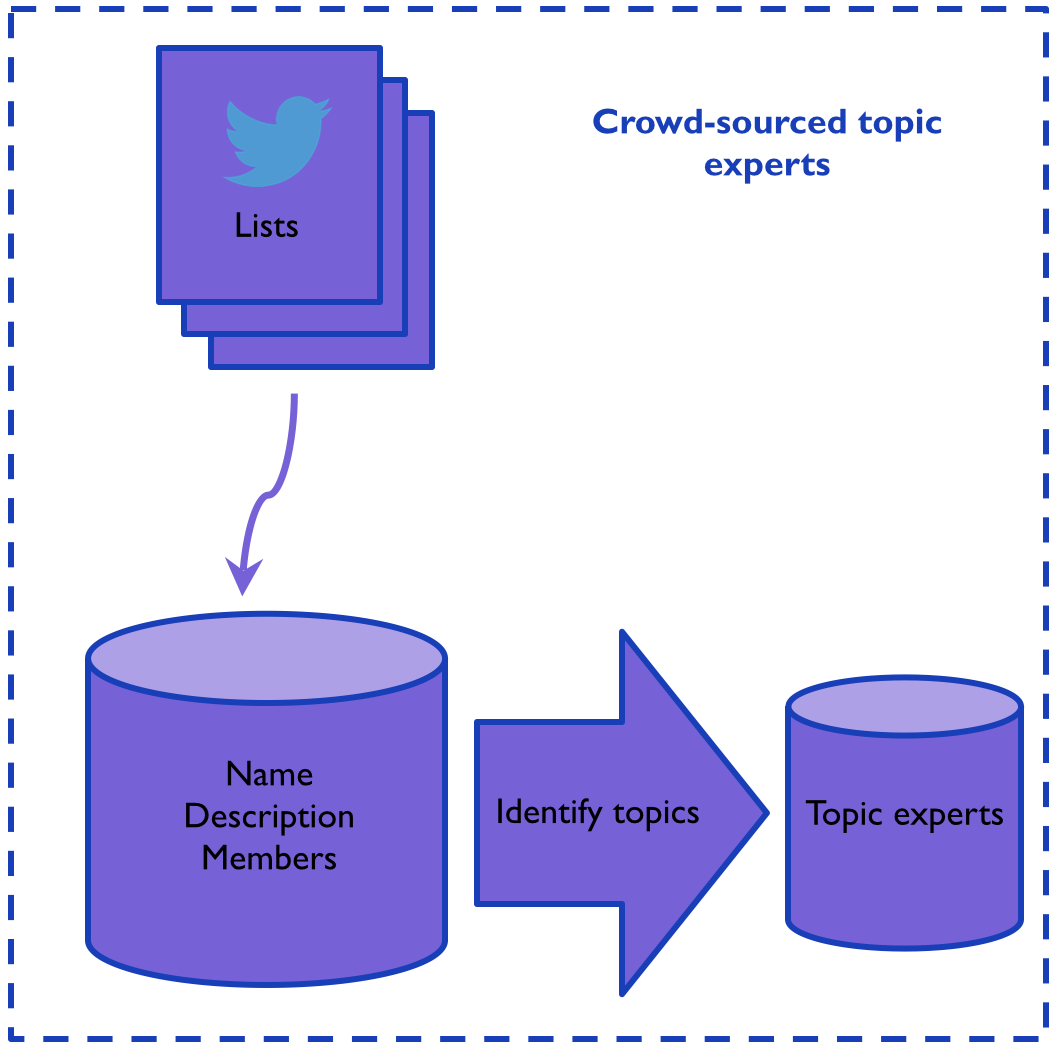
\includegraphics[width=0.8\textwidth]{./IMG/topic_experts.PNG}
	\caption{We check if the user are following any accounts that we have identified as topical experts. We then infer user interest in these topics.}

\end{figure}

In the following section, we discuss our methods for obtaining these three sets of data and describe the technologies we used to do so. 

A key element of our project is Twitter's Lists feature. Lists can be thought of as a way of tagging accounts with identifiers; for example Katy Perry turns up in many ``Music" and ``Pop Star" Lists, while Barack Obama appears in Lists such as ``Influential Figures" and ``Politicians". 


\begin{table}[b!]
    \centering
    \caption{Examples of List members}
    \label{list_names}
        \begin{tabu}{l l X}
        \toprule
        Member                        		& List Name & List Description \\ 
        \midrule
        \multirow{2}{*}{Katy Perry}   	&  Music & Musicians, producers, studio's, record labels\\ \cmidrule(l){2-3} 

                                      			& Music-News-Artists  & Music tweets by artists, labels, fans, organizations, in all - people in the wide world of music.  \\
        			   \midrule

        \multirow{2}{*}{Barack Obama}  &    News \& Politics  &Politicians, current events and news- things to keep me in touch with the world.   \\ \cmidrule(l){2-3} 

                                      			&  Politics & News, Pols, Pundits  \\
	\bottomrule
        \end{tabu}
\end{table}

Lists can be set up by any Twitter user; public Lists can be followed by any user and accessed through the Twitter API. A List has a title, description and multiple members (average of about 300 members per list in our sample). In general, the list name and description relate to the members of the list; we can exploit this fact to identify ``topic experts" - Twitter accounts which have a strong relationship with specific topics (See \cref{list_names} for examples of some Lists and their members).  We drew inspiration from a paper by Ghosh, S, Sharma\cite{cognos}, which details the process of acquiring List data and inferring topics. 

Sharma et al. used three servers that were whitelisted by Twitter, and therefore had almost limitless access to the Twitter API. In addition, they had access to a snapshot of the entire Twitter social graph, which they used to identify hubs and authorities using the HITS algorithm. They could then prioritise loading Lists for the highest-ranked hubs and authorities. Even with these optimisations, Sharma managed to only process a fraction of Twitter Lists. 

\subsection{Inferring User Interest Using Lists}

In 2014 a group from the same Indo-German collaboration published a second paper which outlines a methodology for inferring Twitter users' interests from List data \cite{infer_user_interest}. Due to time and resource constraints, we could not hope to achieve the same results; we decided to prioritise processing the top 1000 Twitter accounts by number of followers. In this way we hope to provide maximum coverage for users of our service. To date we have loaded 600,000 Lists containing \(\sim10\) million unique members, representing around 5\% of the Twitter population.

We load Lists as described above, storing the list id, members, name and description in our database. We then parsed the names and descriptions, removing stop words and domain-specific terms (``Twitter", ``list", ``follows", etc.) and recorded the most frequent terms across all lists. From these top terms, we selected 16 as our topics. With this done, we identify as experts all users who are on 10 or more Lists mentioning our topics. 

\subsubsection*{Inferring User Interest}

\begin{figure}[h]
\centering
	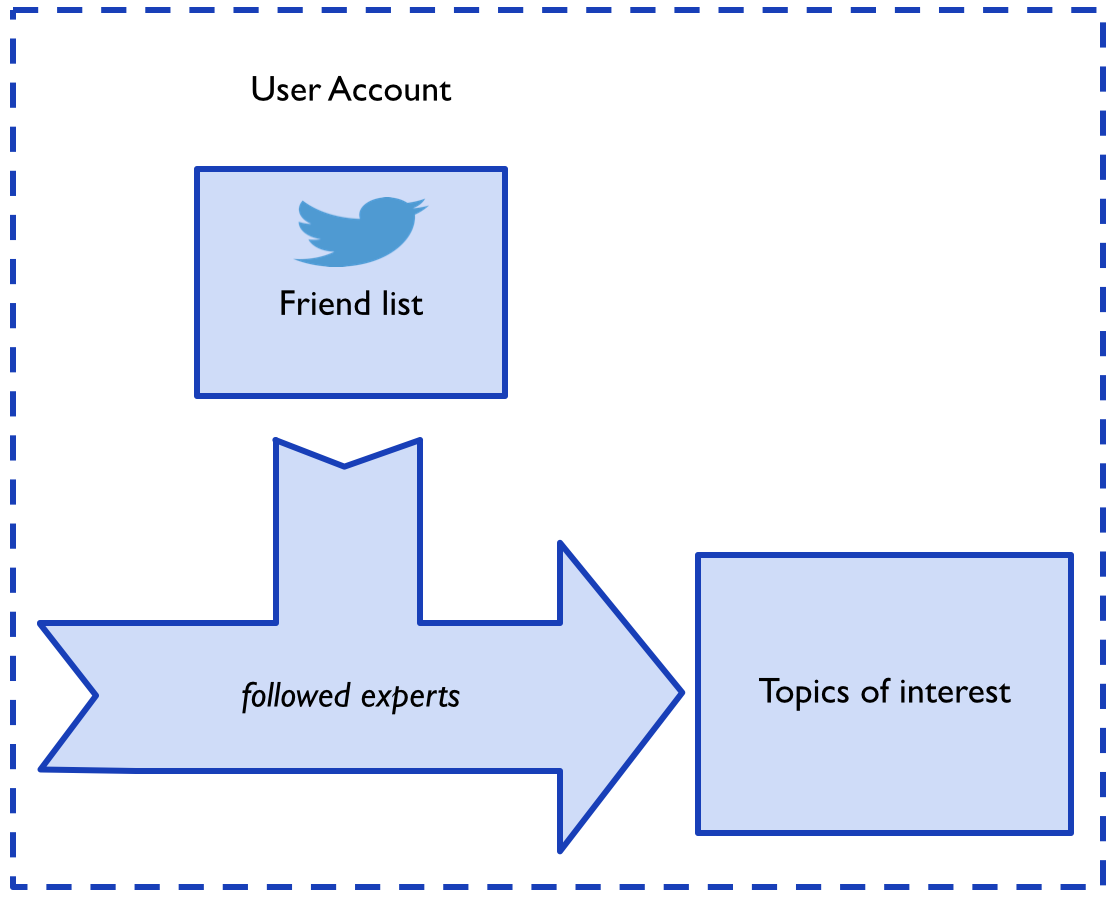
\includegraphics[width=0.8\textwidth]{./IMG/inferring_interest.PNG}
	\caption{We check if the user are following any accounts that we have identified as topical experts. We then infer user interest in these topics.}
	\label{user_interest}

\end{figure}

To identify topics of interest to the user, we first query Twitter for the user's friends' IDs. These are then matched against our expert list, and a Borda count is computed for each expert; the most frequent topic is given a score of 5, the next most frequent a score of 4, etc. These scores are then summed over the entire friend list, giving us a topic distribution for the user. Using this method prevents a bias towards accounts which appear on many lists. (See \cref{user_interest}).

\subsection{Characterising Articles}

We trained a classifier using hand-labelled articles from several RSS feeds; the content of each article was parsed, and a TF-IDF transformation applied. Feature selection was achieved using a linear support vector classifier (SVC), and the transformed data was passed to the classifier.
The classifier we used was a stochastic gradient descent (SGD) classifier with a modified Huber loss function. The classifier was applied in a one-vs-all strategy, fitting each class against all the others. This classifier gave the best results out of several tested, as seen in \cref{compare_classifier}:

\begin{table}[]
\centering
\caption{Comparison of Various Classifiers}
\label{compare_classifier}
\begin{tabu} to \textwidth {X r}
\toprule

\textbf{Classifier} & \textbf{Accuracy} \\
\midrule
Naive Bayes & 0.52 \\
SGD (hinge loss) & 0.73\\
SVC & 0.45\\
SGD (huber loss) & 0.87 \\

\bottomrule
\end{tabu}
\end{table}

\subsection{Recommending Articles}
Three metrics are taken into account when retrieving articles for a user, as follows:
\begin{description}
\item[Twitter Ratings:] The topical interest vector as obtained from the user's Twitter account.
\item[Explicit Ratings:] The user is provided with sliders to adjust the topic rating generated from their Twitter profile or to add and adjust new topics not automatically recommended for them. 
\item[Click-Through Rating:] The number of times the user clicked articles relating to a topic, divided by the number of articles from that topic that they have been shown.
\end{description} 
 
The three vectors are weighted as shown in \cref{recommend}, and the resultant vectors are added and the result normalised to sum to 1. When it comes to recommending articles, we take this topic vector and multiply it by the number of articles we want to retrieve; this gives us a number of articles in each topic proportional to interest in that topic. We then group the article list into equal chunks, such that each chunk has the same distribution of articles as the overall list, and high-ranking topics occur higher up in each chunk. This means that the user will see an immediate change in their feed when they change their profile rating.

\begin{figure}[h]
\centering
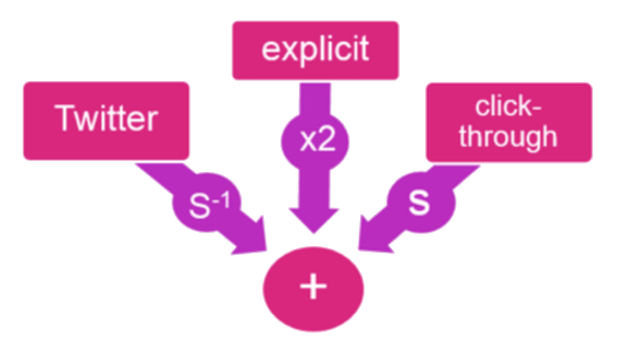
\includegraphics[width=0.8\textwidth]{./IMG/recommend_algo.png}
\caption{The user's explicit feedback is given twice the weight of the other 2 items so that the user sees a response to any feedback given. The purpose of the sigmoid function (S) is to prioritise the Twitter profile information initially, but as the click-through counts are collected, the system will learn more about the user, and the Twitter data will become less important.}
\label{recommend}
\end{figure}

\subsection{User Interface}
The user interface is a simple website with 3 different possible menus on display. The first will display when the user is not logged-in. This is comprised of a Register page, Login page and contact page. The user can sign in if he/she already has an account and register if they do not. Upon login, the user will be presented with the following options:
\begin{description}
\item[My News] displays the user's personalised news feed if they have authorised their Twitter account, and an invitation to do so if they have not. The user enters their details on Twitter and authorises our app to use their account; Twitter will then redirect back to our site.
\item[My Profile] allows users to edit profile information such as password and email as well as other details after the Twitter profile is created.
\end{description}

After the user has authorised our application with Twitter, the following options will be made available: 
\begin{description}
\item[Analytics] gives users an insight into how their profile was generated. Various statistics are displayed here, such as which topics our system identified as being relevant to the user.
\item[My Profile] will now allow users to directly influence their news recommendations if they wish to do so, by adding or removing topics from their profile.
\end{description}

\subsection{Technology Stack}
We used Python for the majority of this project, using Django for handling requests and general web processes and various other packages fulfilling processing roles on the back end. Some of the more important packages we used include:
\subsubsection*{Django Registration Redux}
 This package provides a convenient framework for maintaining user profiles, and made setting up registration, login, signups very straightforward. The registration consists of a simple register step, that allow users to create an account with our site. The Django Registration Redux package comes with many features and provides a number of different pages for all the possible different account related steps in the process such as changing password, account activation, logging in and out and registering.  All of these account related events have a special section for handing these steps and are preceded by ``/account/page.html" to segment the account related events. Registered users can be seen and edited in the administration section in django. 
\subsubsection*{Feedparser \& Newspaper}
These were used in the back end for acquiring content from RSS feeds. The process is follows: the feeds in our database are checked for new articles using Feedparser, the URLs of which are passed on for processing by Newspaper. Newspaper uses a trained model of what the content of an article looks like in a HTML document, which means that it can be used to scrape text from almost any page without the need to use CSS or HTML selectors. 
\subsubsection*{Natural Language Toolkit (NLTK)\cite{nltk}}
Used extensively throughout the project; we wrote a parser for processing List titles and articles using a variety of NLTK's resources (tokenizers, part-of-speech tagging, entity recognition).
\subsubsection*{Tweepy}
This package is a Python wrapper around the Twitter API; we used it for authenticating users with Twitter, obtaining List data and querying user's followed accounts.
\subsubsection*{PostgreSQL}
We used PostgreSQL as our database management system, using a combination of Django models and SQL  commands to interact with the database.

\section{Integration}
\subsection{Integration of System Components}
We feel that we made excellent choices in regards to our technology stack. The PostgreSQL database was well equipped to handle all the various and large data we were storing for this project. Our largest data sets were our Experts and List with over 500k entries each, which PostgreSQL handled with ease. For our front-end we used Bootstrap with a free theme, Andia\cite{andia}. This offered simple and quick scalable design with a flexible framework for the layout of our site. 

For parsing and receiving articles we used feedparser in conjunction with newspaper which complemented each other as we could pass feedparser entire feeds that would in turn pass individual articles to newspaper which would get all the article related information. Wrapping this component in a Celery task running every half-hour ensures that our article database stays up to date.

\subsection{Similarity to Existing Technologies}
Most of the ideas presented in this project have been applied in isolation in an academic setting. For example, the Sharma paper examining the use of Lists for inferring user interest did not discuss its utility in recommending products or news. We discuss here how the topics returned by our system compare to those returned by WhoLikesWhat.
 
\subsubsection{Comparison to WhoLikesWhat}
For each topic in our database, we selected an account suggested by the WhoLikesWhat system \cite{wholikeswhat} and made sure it was covered in the Anthus system (Anthus has less coverage as it only has a small percentage of Twitter Lists). We then compared the top 3 results in the two systems; the results of this evaluation are seen in \cref{wholikeswhatcomparison}. We noted the following during this evaluation:

\begin{enumerate}
\item We registered what we called a ``tech bias'', that is our system identifying a higher level of ``tech'' component than WhoLikesWhat.
\item A better match would have been the word ``movie'' rather than film. Direct text matching will not cope with semantic differences like this.
\item We did not have good matching on sports topics. Again note the semantic difference in the meaning of ``football''.
\end{enumerate}

\begin{table}[]
\centering

\begin{tabu} to \textwidth {@{}l l X X l@{}}
\toprule
Topic & Twitter account  & WhoLikesWhat & AnthusNews	& Notes \\ 
 	 & 			      & (Top 3) 		& (Top 3) 		& \\

\midrule
art           & @tate            & art, culture, design              & art, design, tech           &       \\
business      & @FT              & politics, finance, media            & business, tech               & 1     \\
celebrity     & @JimCarrey       & celebrity, entertainment, actors    & entertainment, celebrity, art &       \\
design        & @mashable        & media, tech, design                 & tech, design                 &       \\
education     & @edutopia        & education, news, media              & education                   &       \\
entertainment & @theellenshow    & celebrity, entertainment, TV        & entertainment, art, music     &       \\
fashion       & @StellaMcCartney & fashion, design, news               & fashion, design              &       \\
film          & @kevinspacey     & entertainment, movies, celebrities  & entertainment, art, film      & 2     \\
food          & @Bourdain        & celebrity, entertainment, foodies & food, entertainment, travel &       \\
health        & @MichaelPollan   & food, health, news                  & food, health, tech            &       \\
music         & @justinbieber    & music, movies, celebrity            & music, art                  &       \\
politics      & @whitehouse      & politics, gov, news                 & politics, tech               & 1     \\
science       & @newscientist    & science, journalists, tech          & tech, science               & 1     \\
sport         & @nfl             & sports, players, football           & sport                       & 3     \\
technology    & @ijustine        & socialmedia, youtubers, tech        & tech, design, music           &       \\
travel        & @lonelyplanet    & travel, blogger, media              & travel                      &       \\ 
\bottomrule
\end{tabu}

\caption{Comparison with WhoLikesWhat}
\label{wholikeswhatcomparison}
\end{table}

\section{Impact}

Anthus News Mission Statement:
\begin{center}
\textit{Provide a diverse and centralised news feed, with quick profile creation that offers the general user a personalised and unique user experience.}
\end{center}
Our site will offer users a new and exciting way to consume relevant news. It will present any potential user with the opportunity to create a more interesting and personalised news feed virtually instantly. 
We aim to create a far more accurate and personalised experience for users through linguistic analysis and advanced premeditated methodologies. Our system will have an impact based upon our research into the most effective processes implemented and studied in previous academic and practical settings. 

We expect it will make an immediate impact when it is released in production. The intended ease of use and simplicity make it immediately useful and accessible with its modularity making it very scalable allowing for future growth and development. The design allows for many features to be added while still being useful in its current minimalistic state. 

We would expect peer recommendations to quickly expand demand for the app. Anthus News is also available on mobile so we would see that as an additional channel for recruiting users. Our promotion of Anthus News via Twitter and Facebook should also bring in new users.

\section{Reflections}
\subsection{Successes}
We succeeded in many aspects of our project such as determining user interest via Twitter, giving the user profile flexibility and including varied content. We compared the topics returned by our system to those suggested by WhoLikesWhat\cite{wholikeswhat}, the results of which can be seen in \cref{wholikeswhatcomparison}. We see decent agreement with the topics returned, which suggests that, despite the limitations we faced regarding resources and time, we have implemented a successful inference system.

We feel that another success for our project was the fact that we satisfied our design objectives, most notably the analytics and profile features. We received positive feedback on these from the UX survey, and we therefore feel that our target users and personas would be satisfied with the system.

On the other hand, the classification of articles was not entirely successful. While training the classifier, we performed k-fold cross-validation on our training data. This produced an accuracy of around 87\%; however, when we inspected the performance of the classifier on real data, we found that the overall accuracy was closer to 70\%. The results from this informal evaluation can be seen in \cref{classifier_performance} The classification of articles is probably the least successful component of the system; this is due to several factors, namely:
\begin{itemize}
\item The topics we selected from the Twitter Lists are too broad, with large overlaps between them. 

\item Our training set was too small (20-30 articles per topic)
\end{itemize}
While these classification issues affect the performance of our system, they could be rectified by simply spending more time training the classifier. In a full-scale version of the system, we would also generate more topics from Lists, and potentially introduce a topic hierarchy to deal with the overlaps between topics. 
A more sophisticated approach to identifying topical experts, perhaps by clustering Lists based on their membership, might also improve the classification. This could also mitigate the effects of synonymous List topics such as ``film'' and ``movies'' as well as polysemous terms such as (American) football and football (soccer).

\begin{table}[h]
\centering
\caption{Classifier Performance per Topic}
\label{classifier_performance}
\begin{tabu} to 0.5\textwidth {@{} lll | lll@{}}
\toprule
Topic         & Rating &False Positives & Topic     & Rating &False Positives \\ \midrule
Art           & 100\%  &                             & Business  & 40\%   & sport                       \\
Entertainment & 70\%   & sport                       & Celebrity & 50\%   & sport, tech                 \\
Music         & 55\%   & sport                       & Tech      & 70\%   & design                      \\
Education     & 75\%   &                             & Film      & 70\%   & sport, celebrity            \\
Science       & 65\%   &                             & Sport     & 100\%  &                             \\
Design        & 40\%   & sport                       & Food      & 90\%   &                             \\
Politics      & 75\%   &                             & Travel    & 50\%   & range of topics             \\
Fashion       & 100\%  &                             & Health    & 55\%   & business                    \\ \bottomrule
\end{tabu}
\end{table}


\subsection{Challenges}
Getting started and organised was a big challenge at the outset. We spent a lot of time talking and discussing all the different directions the project could go in. The initial stages of the project were mainly spent researching different methods for inferring user interests; we feel that this time was spent well, as once we began writing code, we had a clear idea of what needed to be done, and gave us focus for our first minimal viable products.

Overcoming the Twitter rate limits was another challenge initially; Twitter only allows 15 API calls to get a user's List memberships in a 15-minute window. This is clearly insufficient to aggregate the large number of Lists we required. We circumvented this by applying for 10 developer keys, and switching between them when we exceeded the rate limits. This ensured that we had a constant stream of incoming List data. 

We were quite successful when managing the project and task involved in creating the software. We started off with an agile Scrum approach using Trello as a task manager for the first half of the project. We divided up the tasks, self-delegated and completed them in our own time which worked well as many of us were busy during the beginning of the project. As the project progressed, we became more available which allowed us to have regular face-to-face meetings; we decided on various tasks in the morning, communicating and collaborating throughout the day. We had a set plan of what needed to be achieved within increments of 2 week periods much like a sprint.

This style of project management worked well for us, as it allowed us to throw out ideas and discuss them as a team, and all members had a clear vision of our progress at all times.

\subsection{Lessons Learned}
We learned many new technologies such as Python and all the available associated libraries, PostgreSQL, Bootstrap, HTML, CSS, Javascript and jQuery among others. We all learned some skills from each other coming from a diverse background with nobody coming directly from a computer science undergraduate course. Katharine and Kang came from an Engineering background while Liam and James came from Media and Physics respectively. In addition, we had studied a wide variety of subjects between us during the previous semesters. This brought greatly-varying skills and approaches that contributed to the planning, research, implementation and presentation aspects of the project.

\bibliographystyle{unsrt}
\bibliography{references.bib}

\end{document}